\scanpage{152}
Autres foncteurs canoniques sur $\mathcal M$ : foncteurs de Hodge, de \deleted{\unsure{Hodge}} De Rham (fidèles en car. $0$), de Betti (si $k=\mathbf C$)\deleted{\unsure{k}}. Il y a d'ailleurs des structures supplémentaires importantes à mettre sur ces foncteurs....

On a un bifoncteur
\diagram{\begin{tikzcd}
\mathcal V\times\mathcal V \arrow[r,dash] & \mathcal V\\
X,Y \arrow[r,rightsquigarrow] & X\times Y
\end{tikzcd}}
qui est associatif et commutatif, d'où une structure \unsure{multiplication|multiplicative} dans $\mathcal M$.
La formule de Künneth en cohomologie implique que $T_\ell$ est un foncteur qui commute \deleted{aux} à l'opération $\otimes$, donc aux opérations tensorielles.

\figure{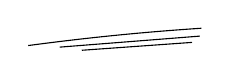
\begin{tikzpicture}[x=1cm,y=1cm]
\draw (0,0) .. controls (0.9,0.12) and (1.6,0.18) .. (2.2,0.22);
\draw (0.4,-0.02) -- (2.18,0.12);
\draw (0.68,-0.06) -- (2.08,0.04);
\end{tikzpicture}}

Revenons à la situation abstraite précédente. Nous supposons maintenant que pour tout $X\in\operatorname{Ob}\mathcal V$, on se donne des \inserted{\uline{projecteurs}} $\pi_i\in\operatorname{Fl}(X,X)$ $(i\in\mathbf N)$, \inserted{presque tous nuls,} de somme $1$, deux à deux orthogonaux, fonctoriels en
\mspage{151}
